%%%%%%%%%%%%%%%%%%%%%%%%%%%%%%%%%%%%%%%%%
% Beamer Presentation
% LaTeX Template
% Version 1.0 (10/11/12)
%
% This template has been downloaded from:
% http://www.LaTeXTemplates.com
%
% License:
% CC BY-NC-SA 3.0 (http://creativecommons.org/licenses/by-nc-sa/3.0/)
%
%%%%%%%%%%%%%%%%%%%%%%%%%%%%%%%%%%%%%%%%%

%----------------------------------------------------------------------------------------
%	PACKAGES AND THEMES
%----------------------------------------------------------------------------------------

\documentclass{beamer}

\mode<presentation> {

% The Beamer class comes with a number of default slide themes
% which change the colors and layouts of slides. Below this is a list
% of all the themes, uncomment each in turn to see what they look like.

%\usetheme{default}
%\usetheme{AnnArbor}
%\usetheme{Antibes}
%\usetheme{Bergen}
%\usetheme{Berkeley}
%\usetheme{Berlin}
%\usetheme{Boadilla}
%\usetheme{CambridgeUS}
%\usetheme{Copenhagen}
%\usetheme{Darmstadt}
%\usetheme{Dresden}
%\usetheme{Frankfurt}
%\usetheme{Goettingen}
%\usetheme{Hannover}
%\usetheme{Ilmenau}
%\usetheme{JuanLesPins}
%\usetheme{Luebeck}
%\usetheme{Madrid}
%\usetheme{Malmoe}
%\usetheme{Marburg}
%\usetheme{Montpellier}
%\usetheme{PaloAlto}
%\usetheme{Pittsburgh}
\usetheme{Rochester}
%\usetheme{Singapore}
%\usetheme{Szeged}
%\usetheme{Warsaw}

% As well as themes, the Beamer class has a number of color themes
% for any slide theme. Uncomment each of these in turn to see how it
% changes the colors of your current slide theme.

%\usecolortheme{albatross}
%\usecolortheme{beaver}
%\usecolortheme{beetle}
%\usecolortheme{crane}
%\usecolortheme{dolphin}
%\usecolortheme{dove}
%\usecolortheme{fly}
%\usecolortheme{lily}
%\usecolortheme{orchid}
%\usecolortheme{rose}
%\usecolortheme{seagull}
%\usecolortheme{seahorse}
%\usecolortheme{whale}
%\usecolortheme{wolverine}

%\setbeamertemplate{footline} % To remove the footer line in all slides uncomment this line
%\setbeamertemplate{footline}[page number] % To replace the footer line in all slides with a simple slide count uncomment this line

\setbeamertemplate{navigation symbols}{} % To remove the navigation symbols from the bottom of all slides uncomment this line

\definecolor{OUGold}{RGB}{181,154,57}
\setbeamercolor{structure}{fg=OUGold}
\setbeamercolor{block title example}{bg=OUGold}
\setbeamercolor{section in toc}{fg=black}

% position the logo
\addtobeamertemplate{frametitle}{}{%
	\begin{textblock*}{\paperwidth}(290pt,-38pt)
		
\includegraphics[height=1cm,keepaspectratio]{sail}
	\end{textblock*}}
}

\usepackage{textpos} % package for the positioning
\usepackage{graphicx} % Allows including images
\usepackage{booktabs} % Allows the use of \toprule, \midrule and \bottomrule in tables
\usepackage{pdfpages} % Allows including PDFs (in separate frame)

%----------------------------------------------------------------------------------------
%	TITLE PAGE
%----------------------------------------------------------------------------------------

\title[Bank Marketing Project]{Bank Marketing Project: Presentation 2} % The short title appears at the bottom of every slide, the full title is only on the title page

\author{Evan Bradley} % Your name
\institute[OU] % Your institution as it will appear on the bottom of every slide, may be shorthand to save space
{
Oakland University \\ % Your institution for the title page
\medskip
\textit{edbradley@oakland.edu} % Your email address
}
\date{November 2016} % Date, can be changed to a custom date

\begin{document}

\begin{frame}
	\frametitle{\space}
	\titlepage % Print the title page as the first slide
\end{frame}

\begin{frame}
\frametitle{Overview} % Table of contents slide, comment this block out to remove it
\tableofcontents % Throughout your presentation, if you choose to use \section{} and \subsection{} commands, these will automatically be printed on this slide as an overview of your presentation
\end{frame}

%----------------------------------------------------------------------------------------
%	PRESENTATION SLIDES
%----------------------------------------------------------------------------------------

%------------------------------------------------
\section{Overview of Process} % Sections can be created in order to organize your presentation into discrete blocks, all sections and subsections are automatically printed in the table of contents as an overview of the talk
%------------------------------------------------

%\subsection{Test} % A subsection can be created just before a set of slides with a common theme to further break down your presentation into chunks

%------------------------------------------------

\begin{frame}
	\frametitle{Overall Process}
  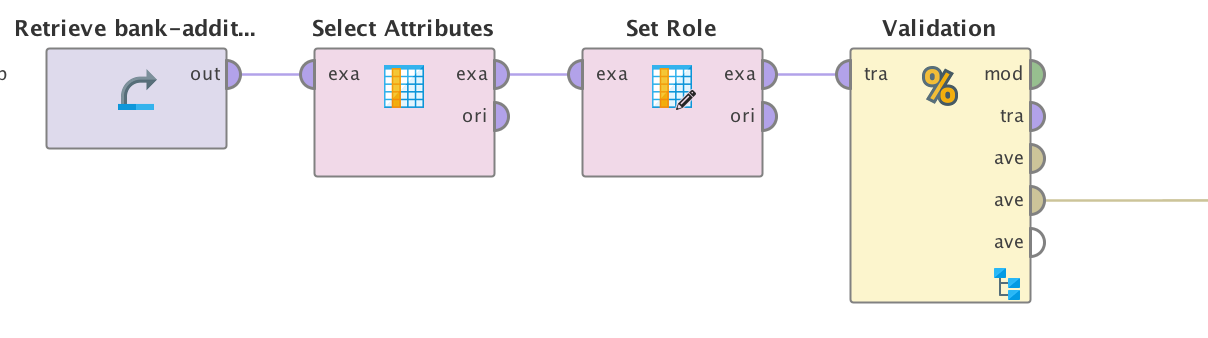
\includegraphics[width=\textwidth,height=\textheight,keepaspectratio]{process}
\end{frame}

\begin{frame}
	\frametitle{Cross-validation Process}
  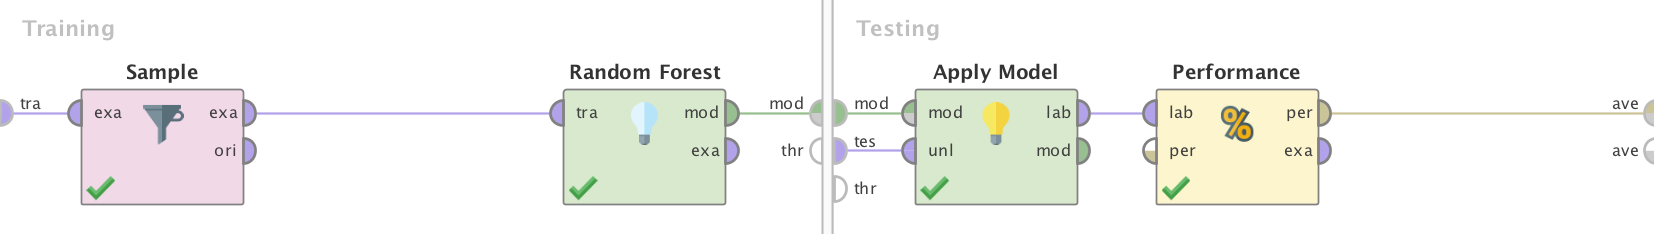
\includegraphics[width=\textwidth,height=\textheight,keepaspectratio]{x-val-process}
\end{frame}

% ------------------------------------------------
\section{Preprocessing} % Sections can be created in order to organize your presentation into discrete blocks, all sections and subsections are automatically printed in the table of contents as an overview of the talk
%------------------------------------------------

\begin{frame}
	\frametitle{Categorical variables}
  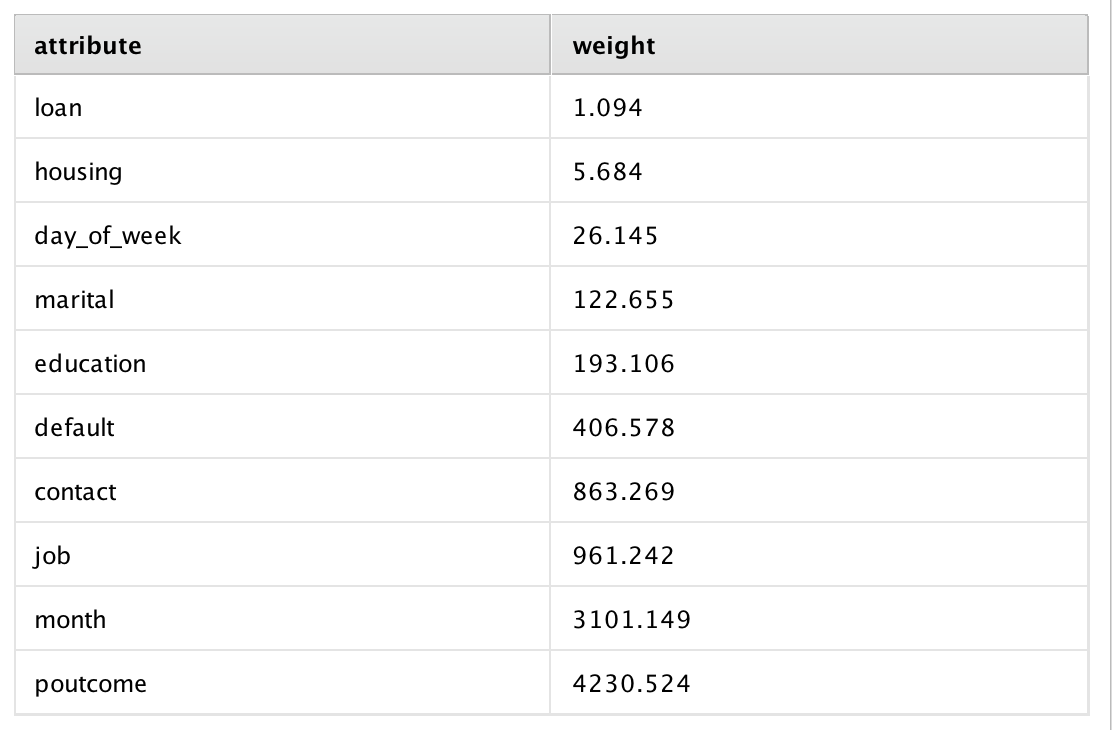
\includegraphics[width=\textwidth,height=\textheight,keepaspectratio]{chi-squared-table}
\end{frame}

\begin{frame}
	\frametitle{Categorical variables}
  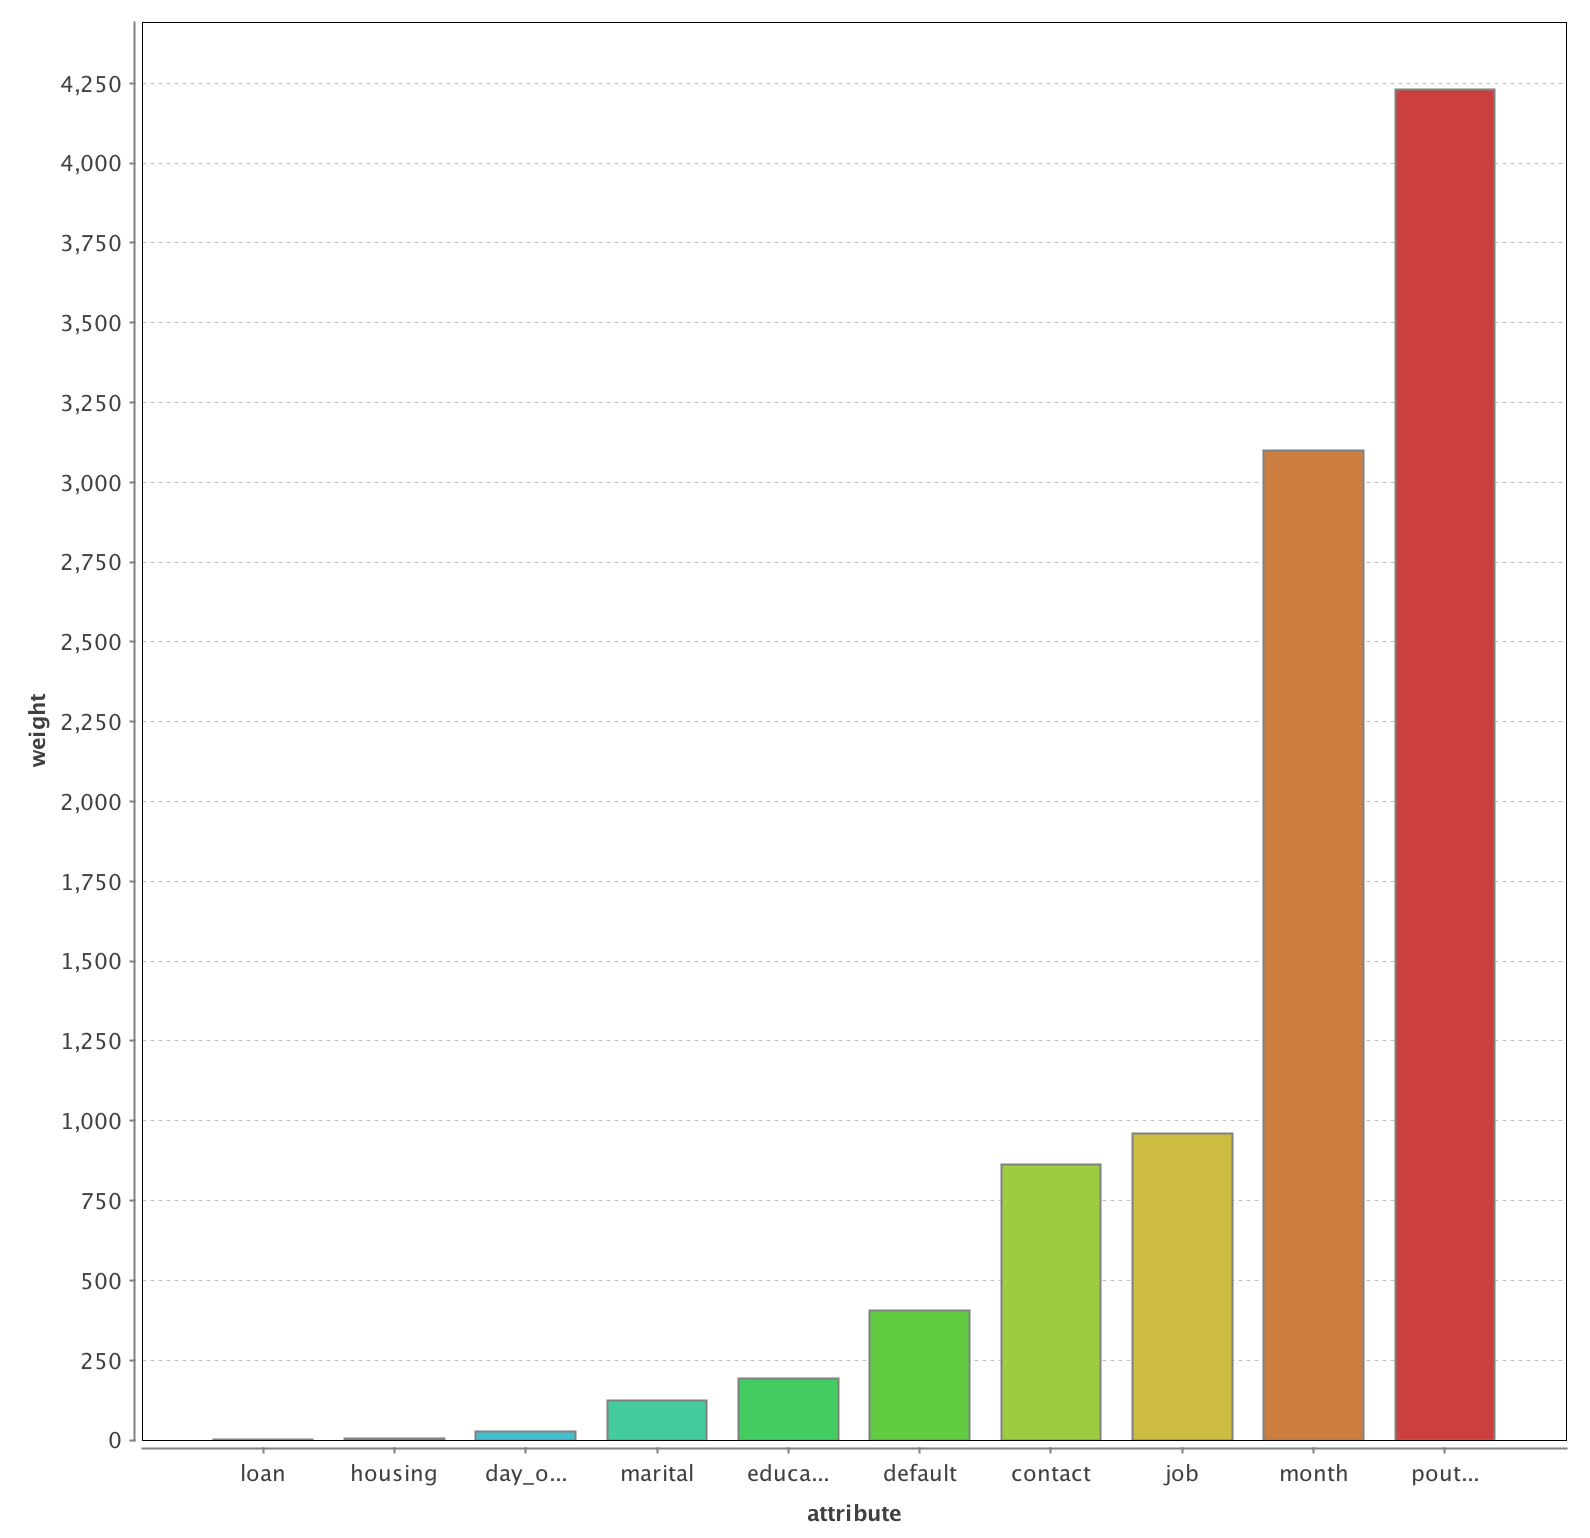
\includegraphics[width=\textwidth,height=\textheight,keepaspectratio]{chi-squared}
\end{frame}

\begin{frame}
	\frametitle{Economic Indicators}
  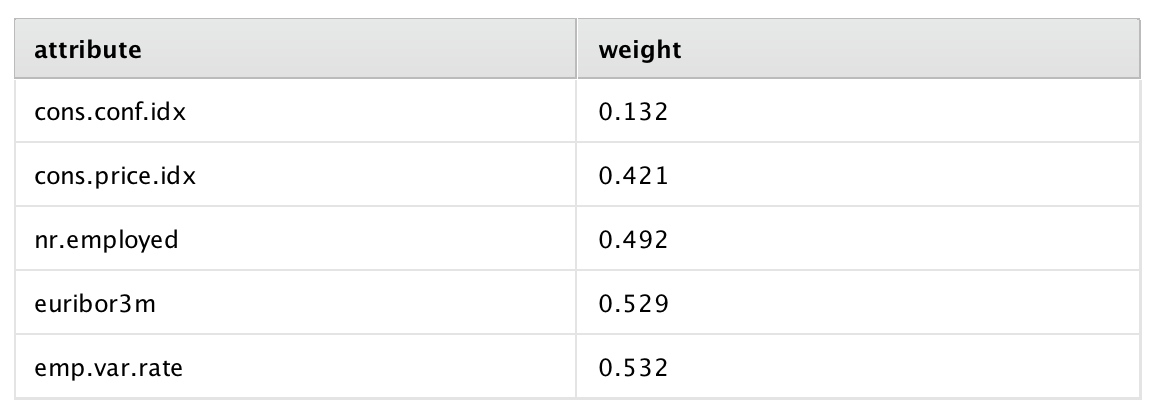
\includegraphics[width=\textwidth,height=\textheight,keepaspectratio]{pca-table}
\end{frame}

\begin{frame}
	\frametitle{Economic Indicators}
  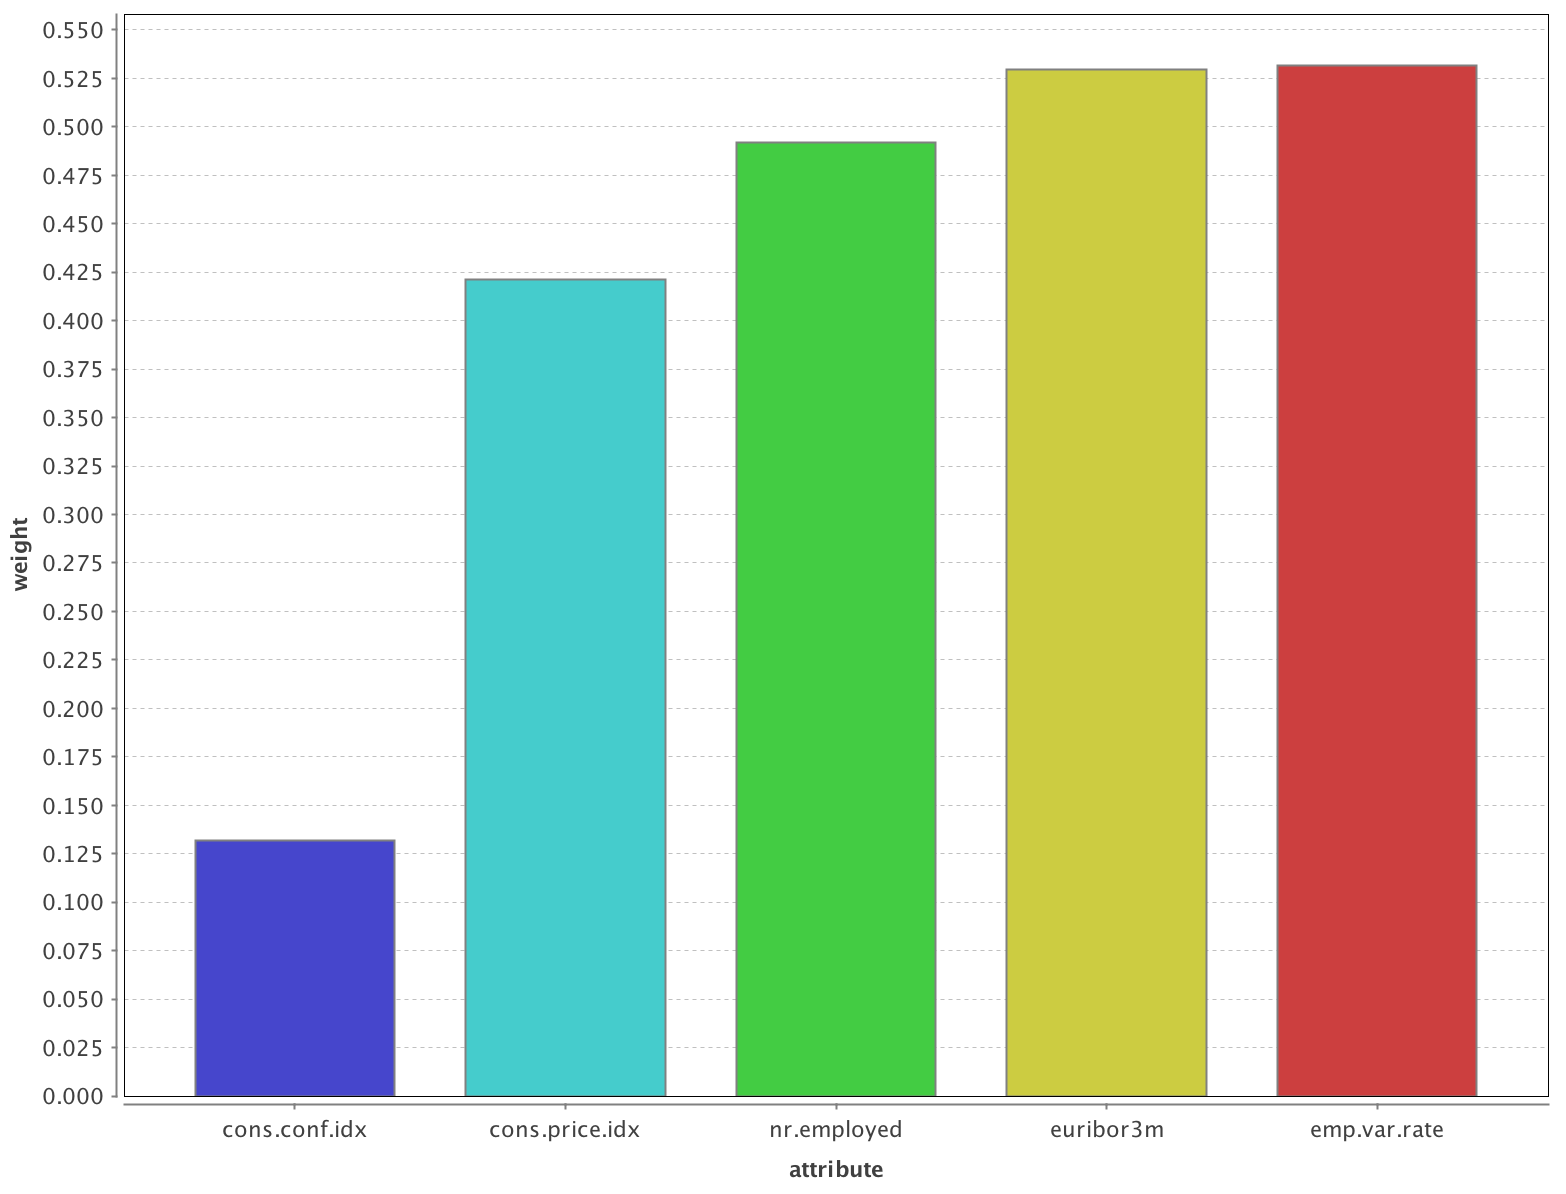
\includegraphics[width=\textwidth,height=\textheight,keepaspectratio]{pca}
\end{frame}

\begin{frame}
	\frametitle{Attribute removal}
  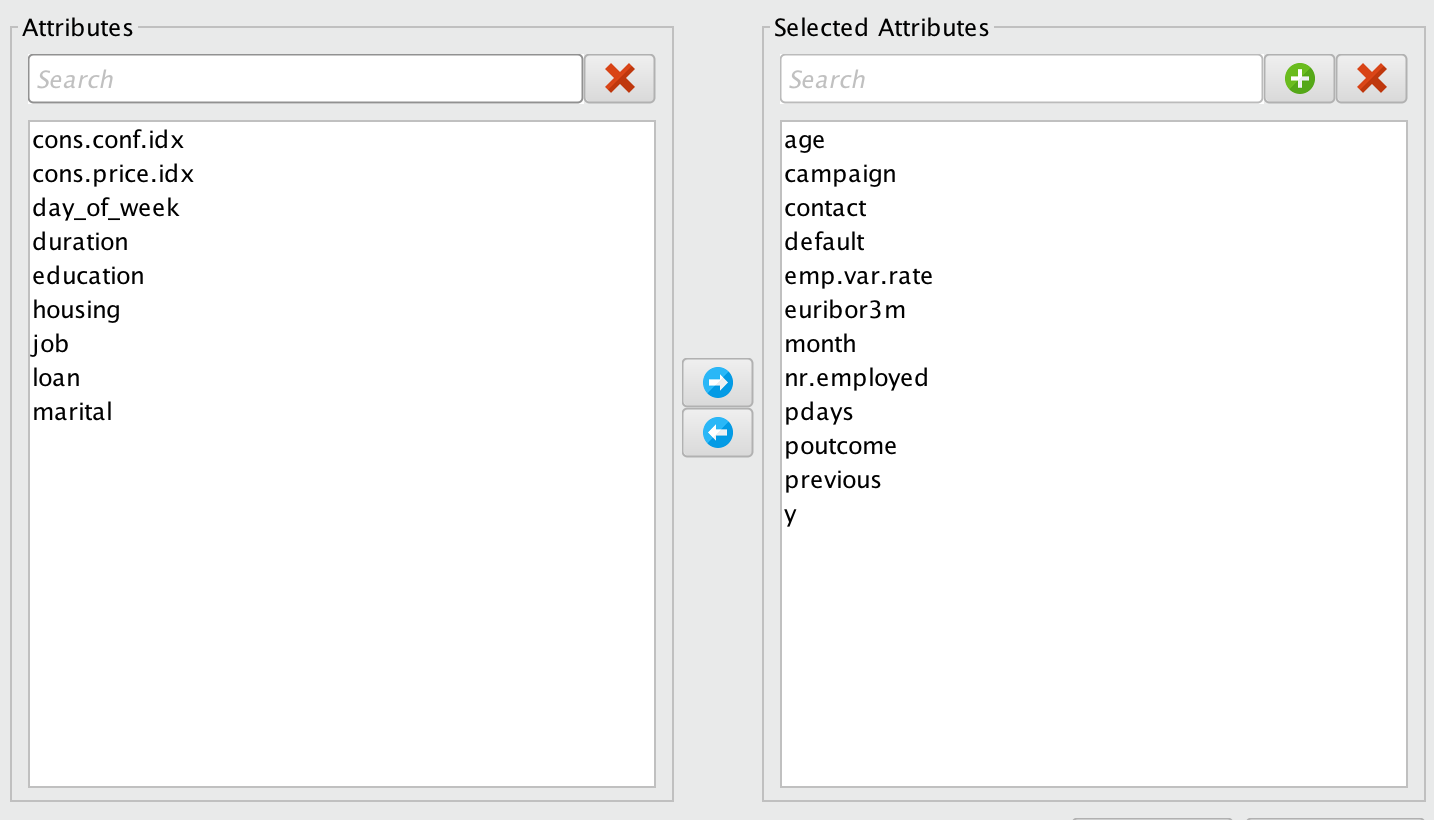
\includegraphics[width=\textwidth,height=\textheight,keepaspectratio]{attributes}
\end{frame}

\begin{frame}
	\frametitle{Sampling}
  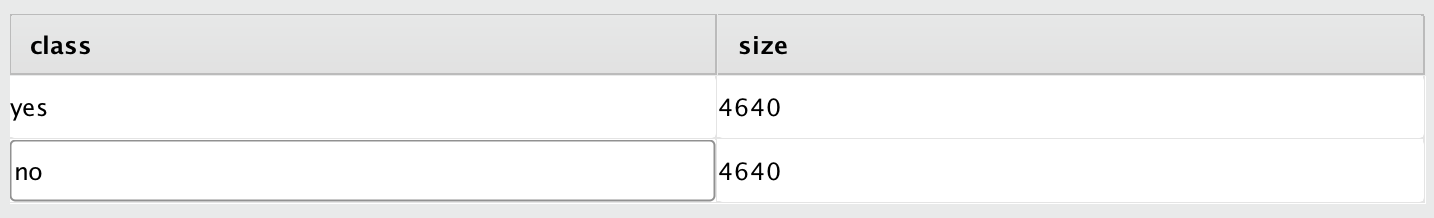
\includegraphics[width=\textwidth,height=\textheight,keepaspectratio]{sample}
\end{frame}

% ------------------------------------------------
\section{Results} % Sections can be created in order to organize your presentation into discrete blocks, all sections and subsections are automatically printed in the table of contents as an overview of the talk
%------------------------------------------------

\begin{frame}
	\frametitle{Decision Tree}
  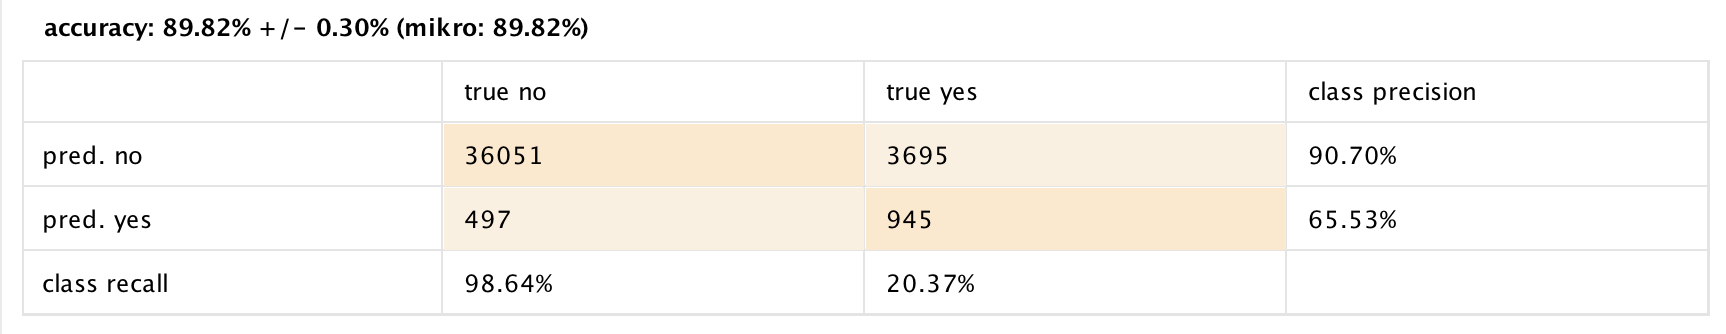
\includegraphics[width=\textwidth,height=\textheight,keepaspectratio]{dt-aa-nos}
\end{frame}

\begin{frame}
	\frametitle{Decision Tree}
  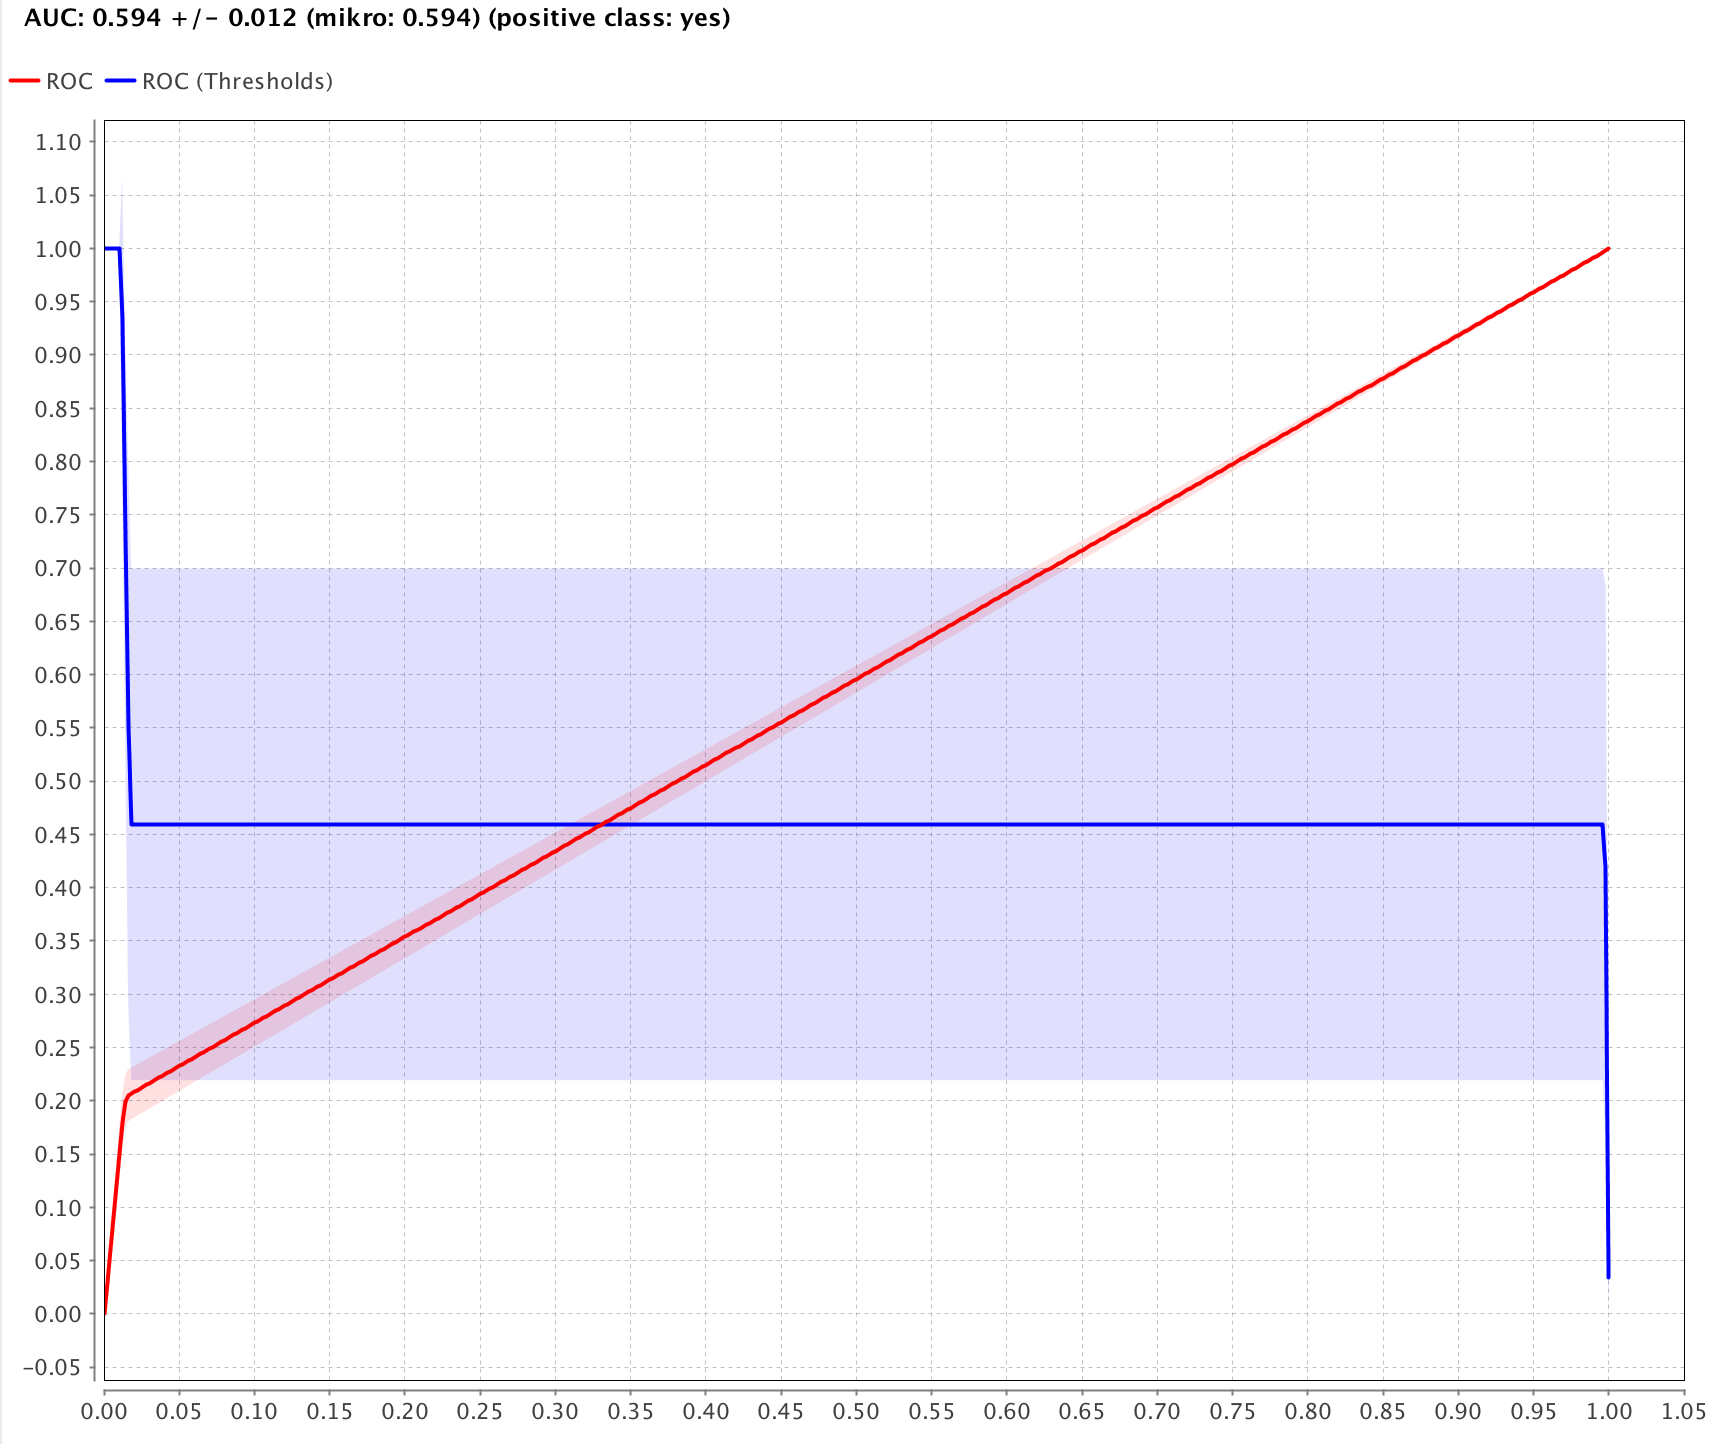
\includegraphics[width=\textwidth,height=\textheight,keepaspectratio]{dt-aa-roc}
\end{frame}

\begin{frame}
	\frametitle{Decision Tree}
  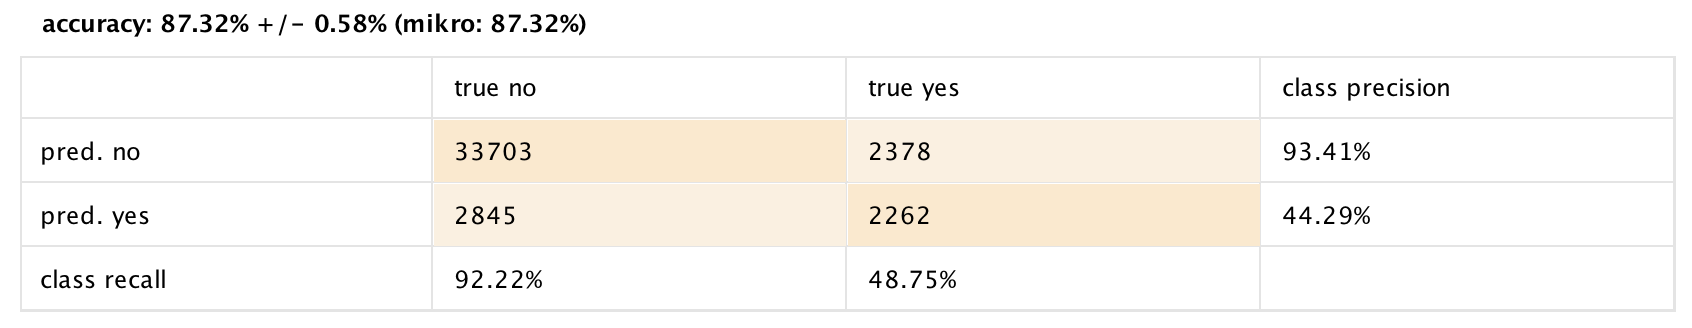
\includegraphics[width=\textwidth,height=\textheight,keepaspectratio]{dt-ra-s}
\end{frame}

\begin{frame}
	\frametitle{Decision Tree}
  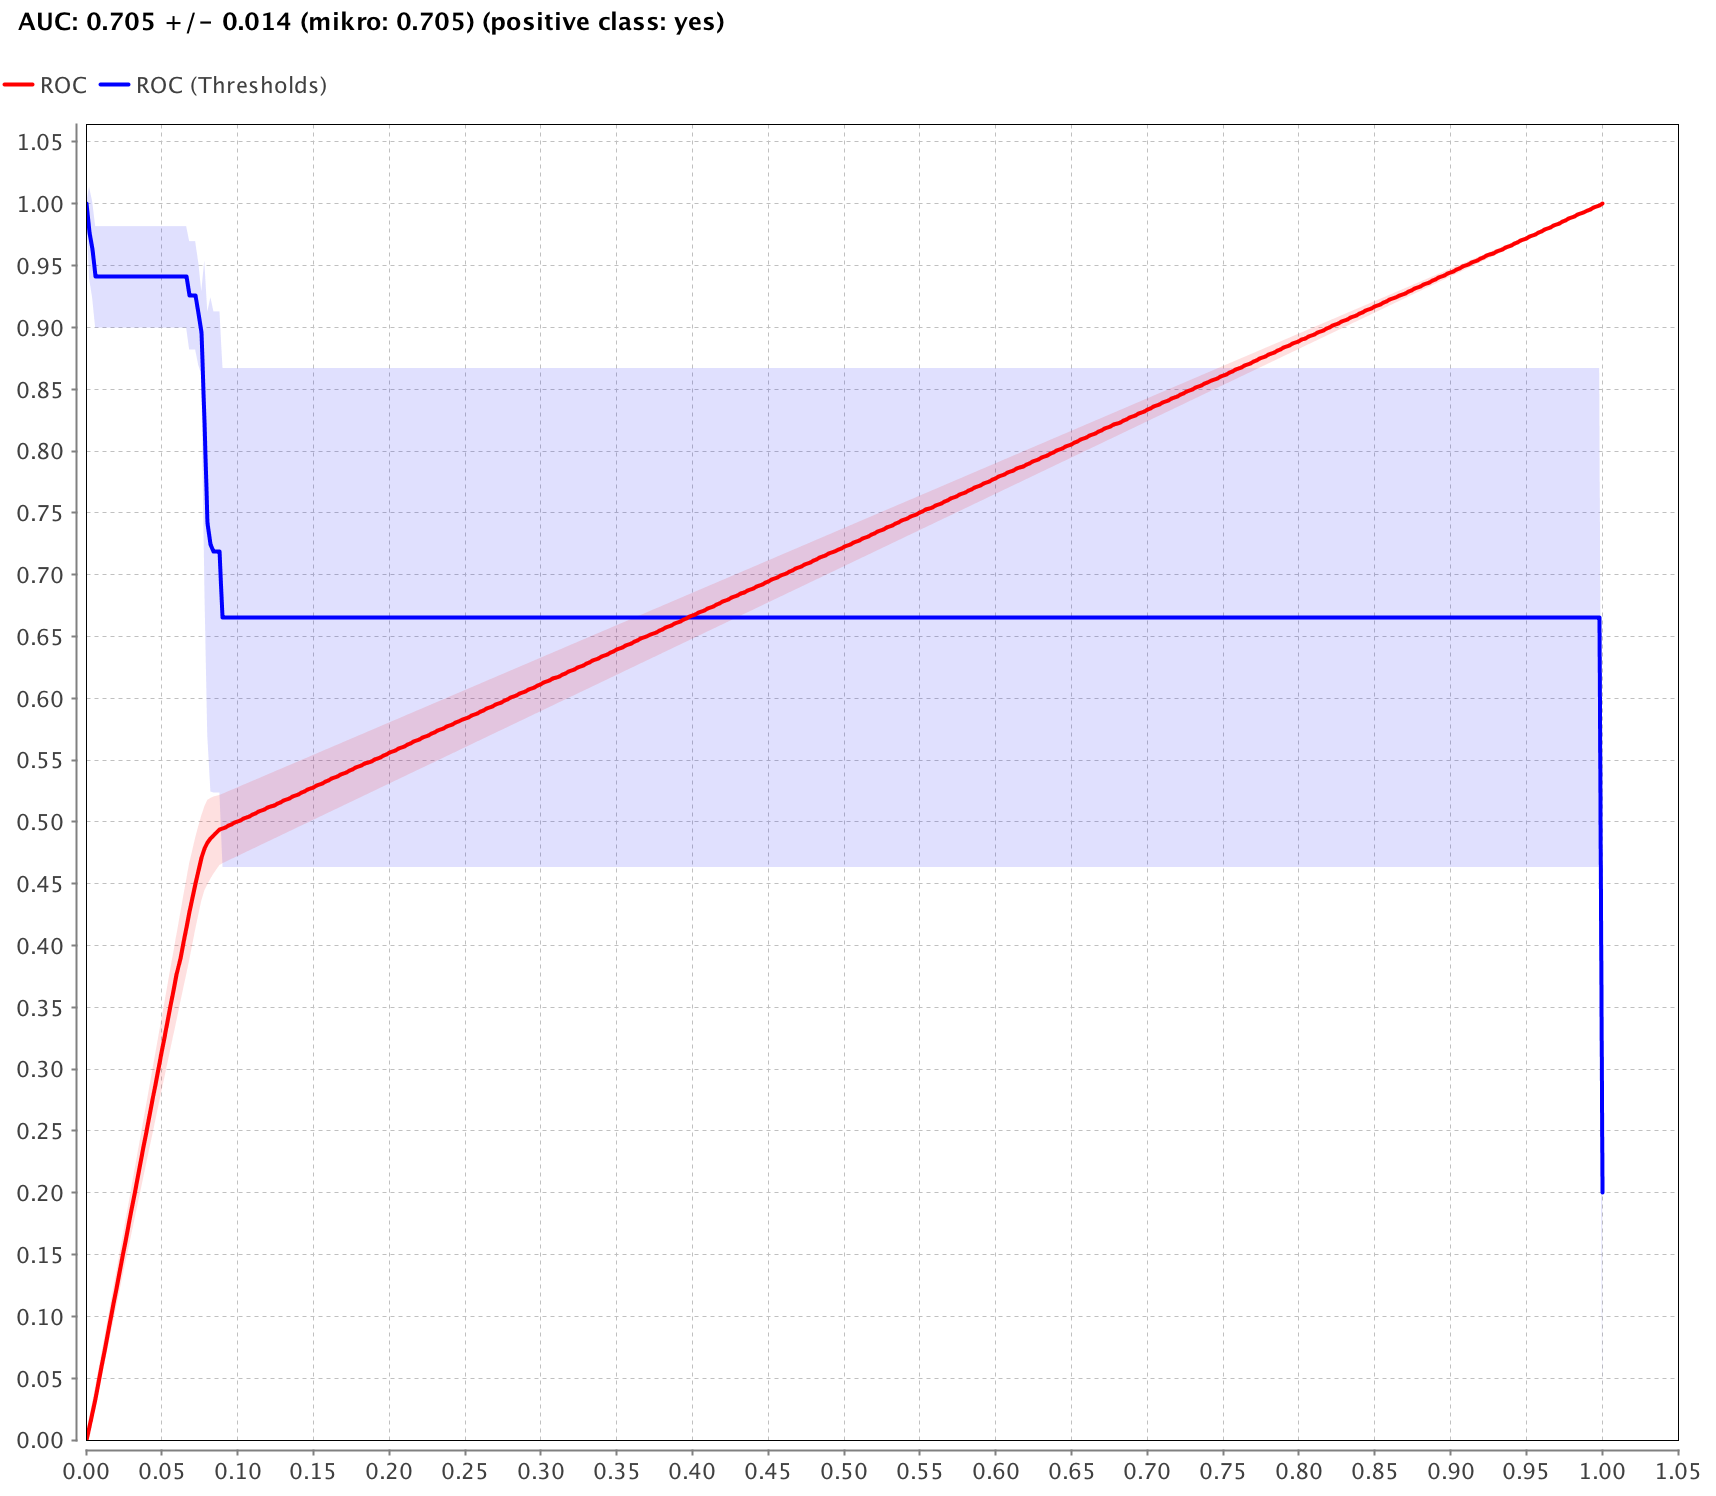
\includegraphics[width=\textwidth,height=\textheight,keepaspectratio]{dt-ra-s-roc}
\end{frame}

\begin{frame}
	\frametitle{Decision Tree}
  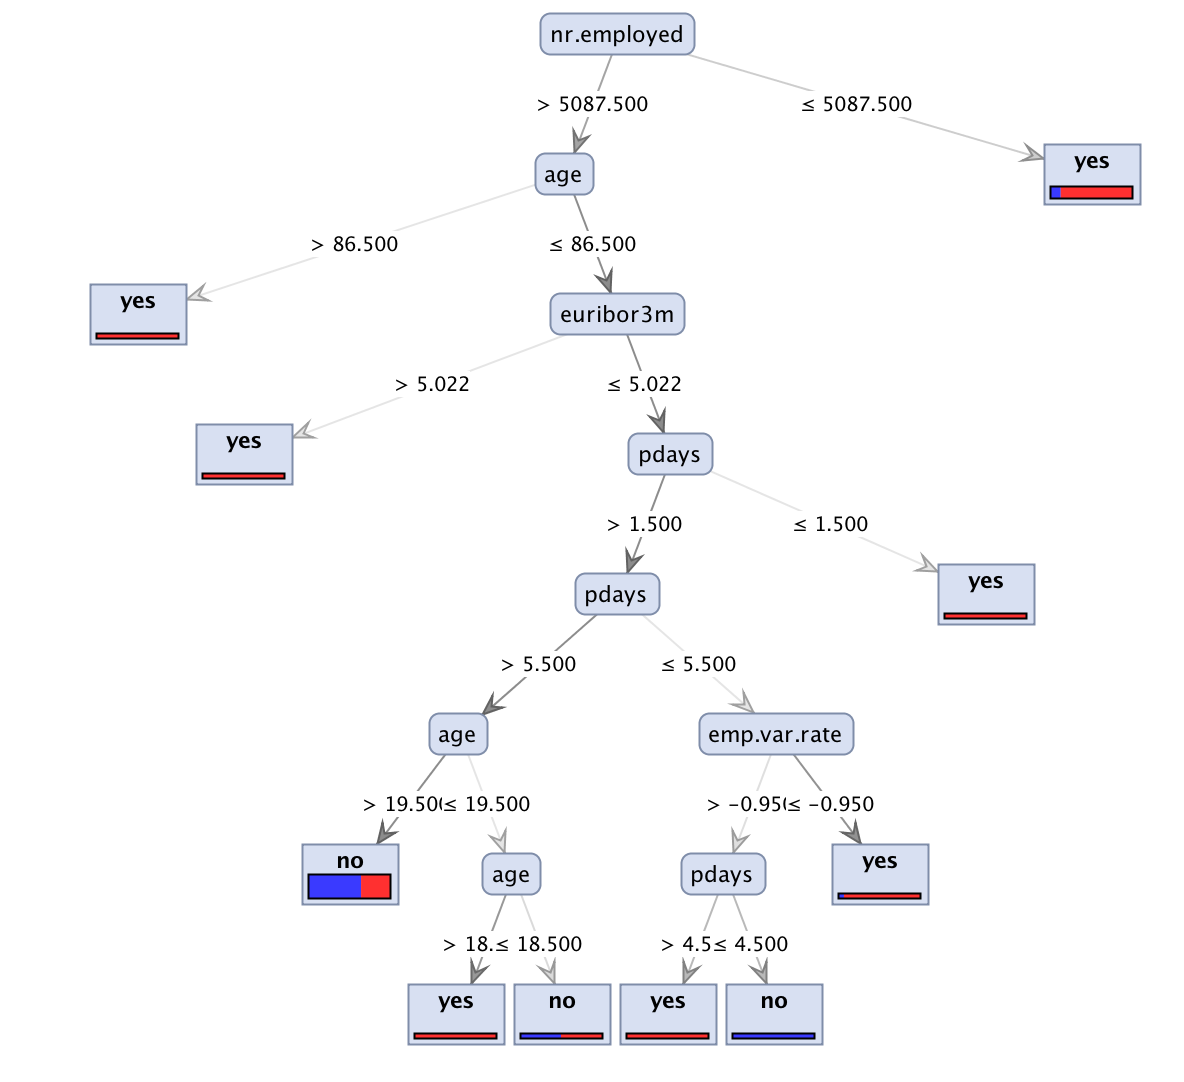
\includegraphics[width=\textwidth,height=\textheight,keepaspectratio]{dt-ra-s-tree}
\end{frame}

\begin{frame}
	\frametitle{Support Vector Machine}
  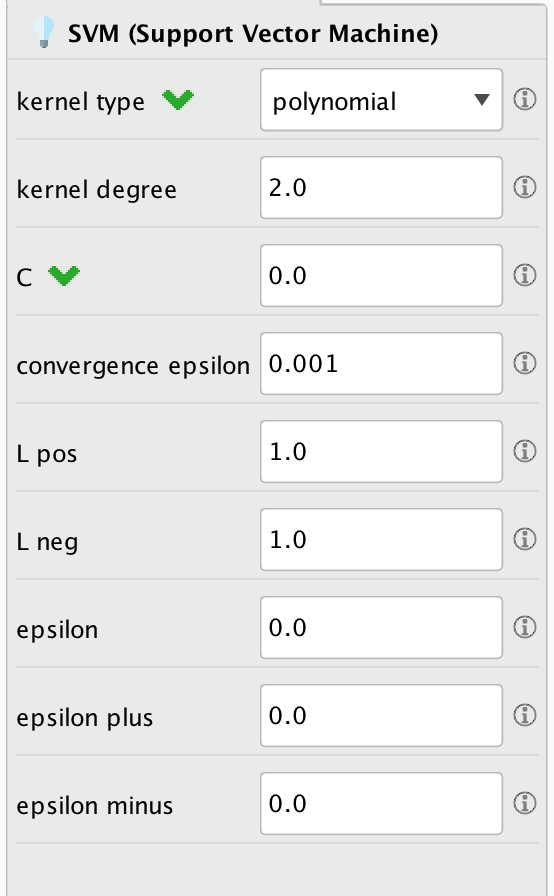
\includegraphics[width=\textwidth,height=\textheight,keepaspectratio]{svm-opt}
\end{frame}

\begin{frame}
	\frametitle{Support Vector Machine}
  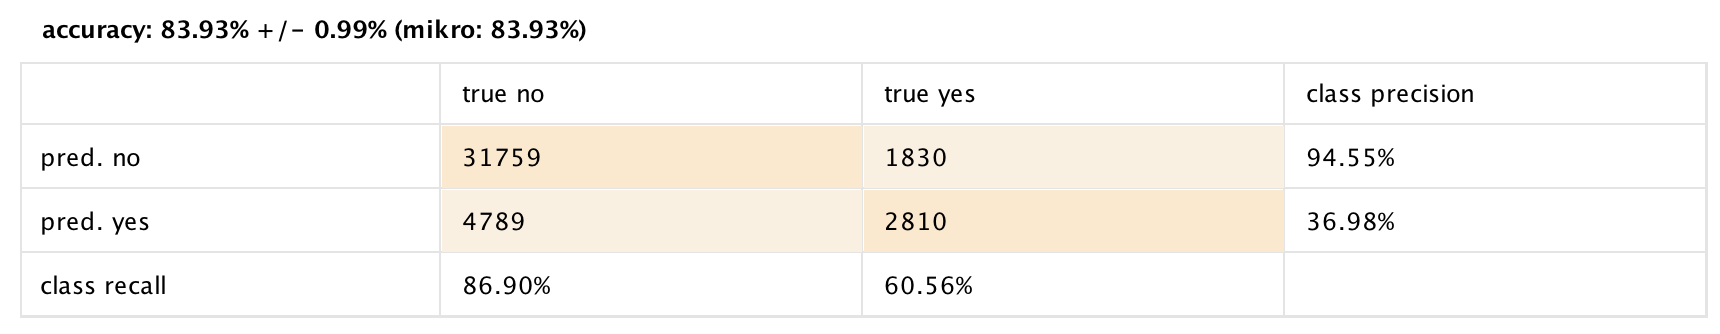
\includegraphics[width=\textwidth,height=\textheight,keepaspectratio]{svm}
\end{frame}

\begin{frame}
	\frametitle{Support Vector Machine}
  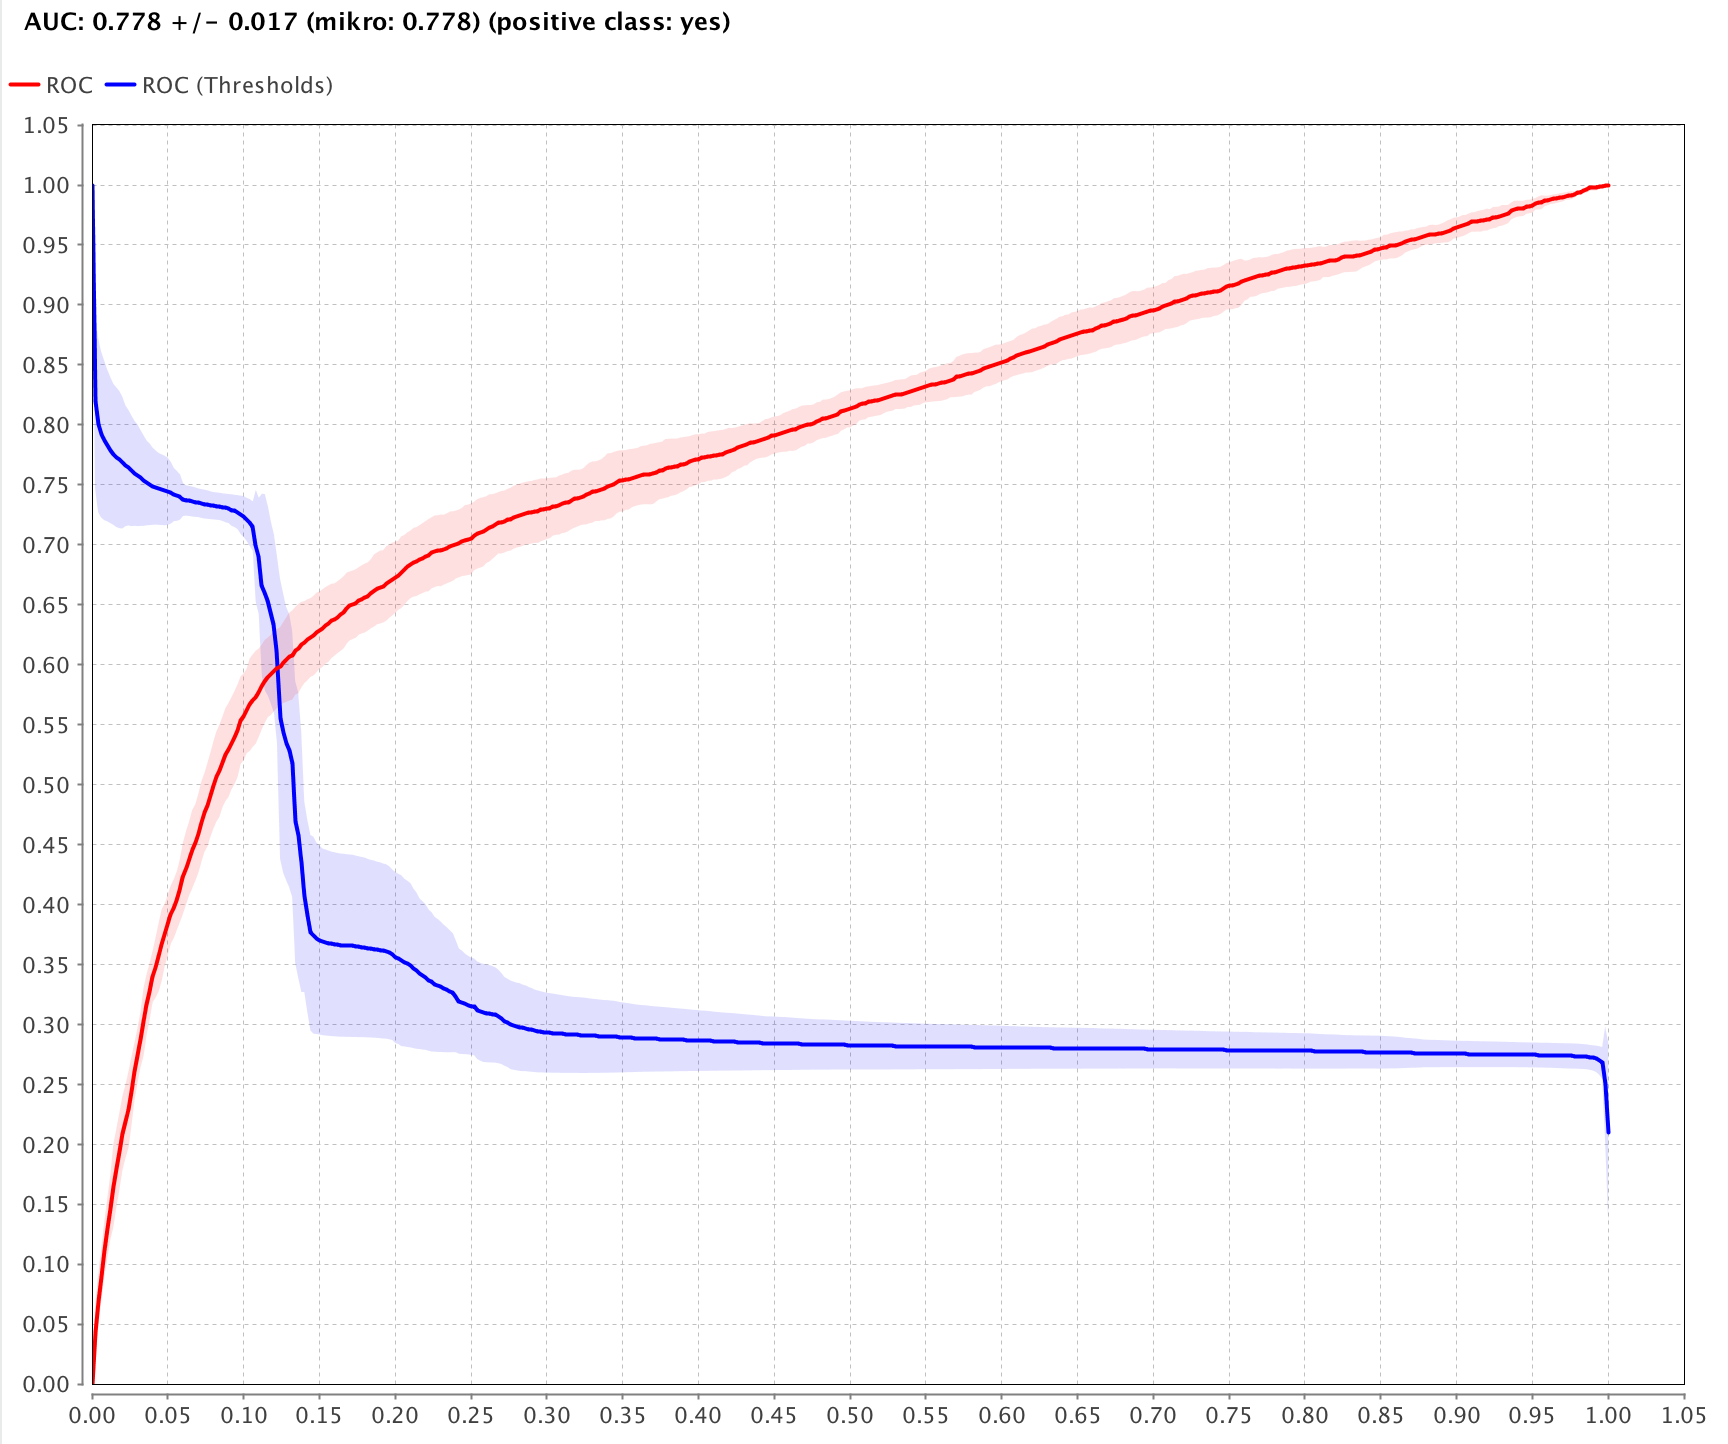
\includegraphics[width=\textwidth,height=\textheight,keepaspectratio]{svm-roc}
\end{frame}

\begin{frame}
	\frametitle{Neural Net}
  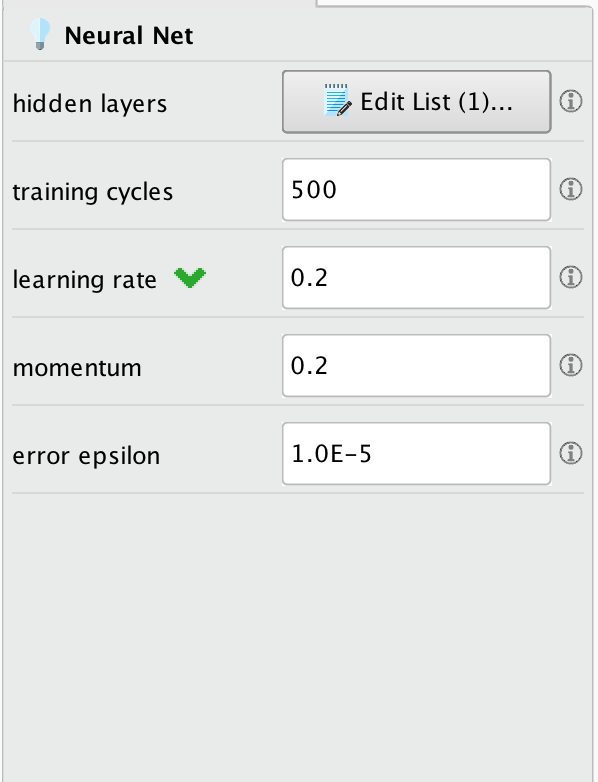
\includegraphics[width=\textwidth,height=\textheight,keepaspectratio]{nn-opt}
\end{frame}

\begin{frame}
	\frametitle{Neural Net}
  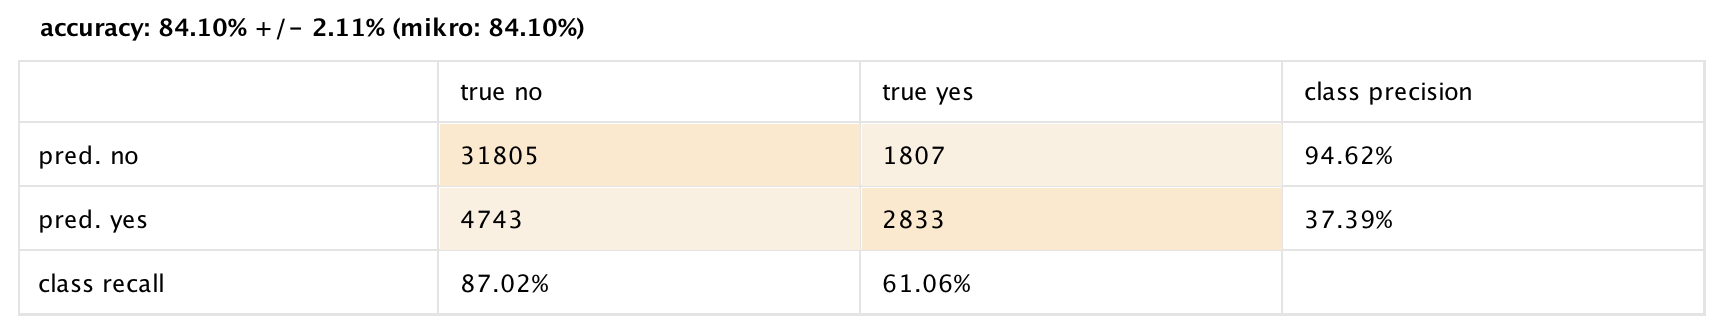
\includegraphics[width=\textwidth,height=\textheight,keepaspectratio]{nn}
\end{frame}

\begin{frame}
	\frametitle{Neural Net}
  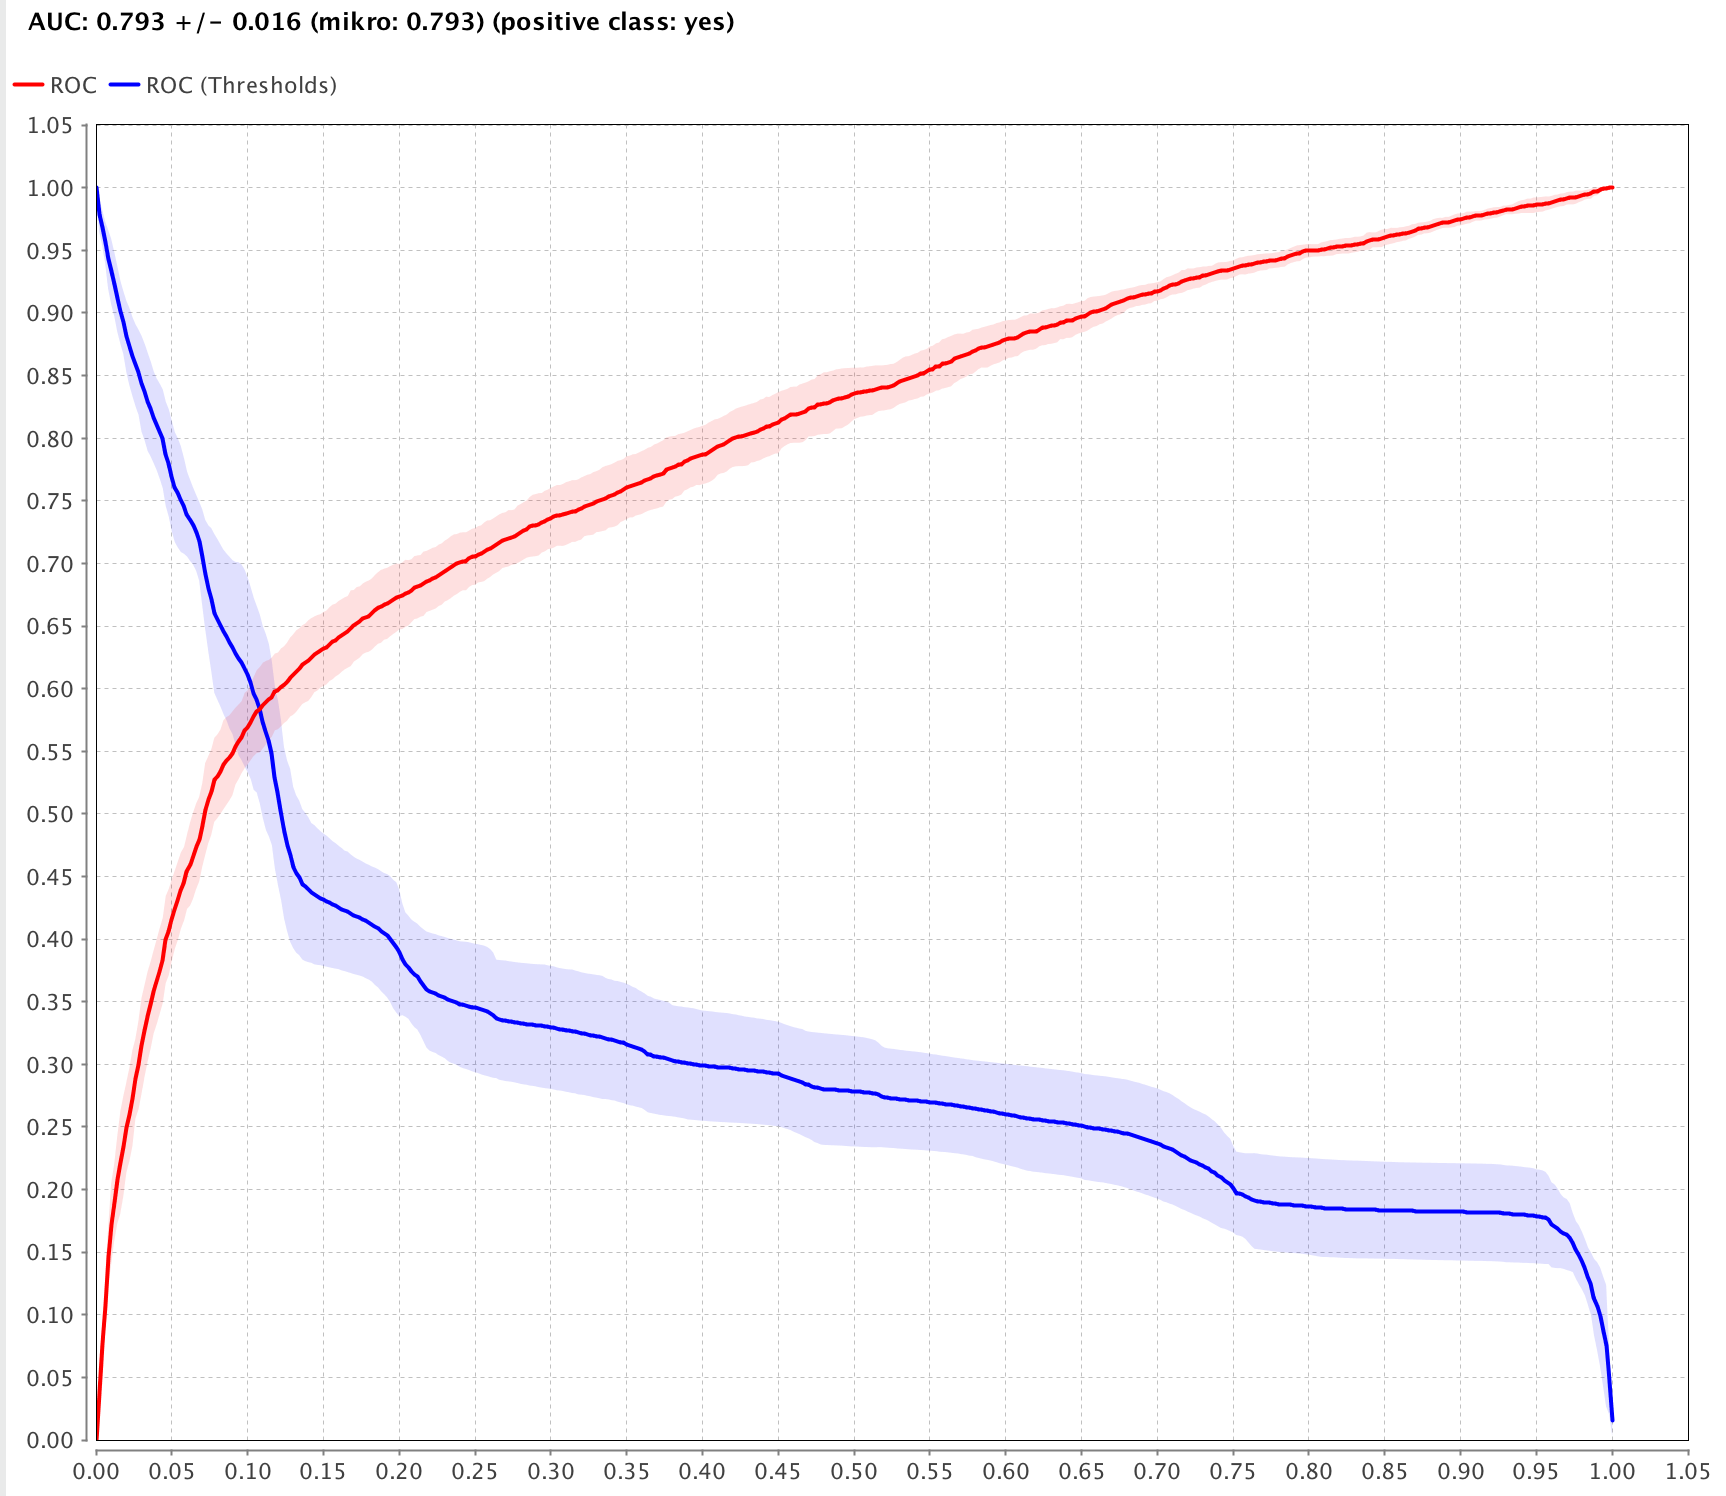
\includegraphics[width=\textwidth,height=\textheight,keepaspectratio]{nn-roc}
\end{frame}

\begin{frame}
	\frametitle{Random Forest}
  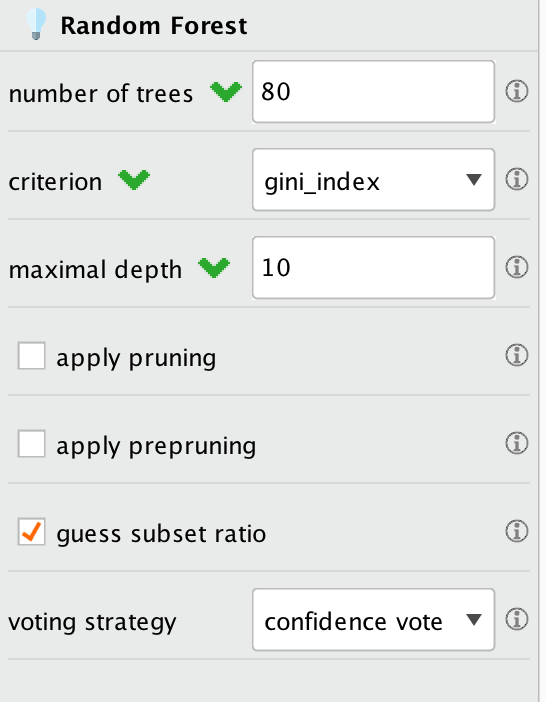
\includegraphics[width=\textwidth,height=\textheight,keepaspectratio]{rand-forest-opt}
  %\includegraphics[width=\textwidth,height=\textheight,keepaspectratio]{}
\end{frame}

\begin{frame}
	\frametitle{Random Forest}
  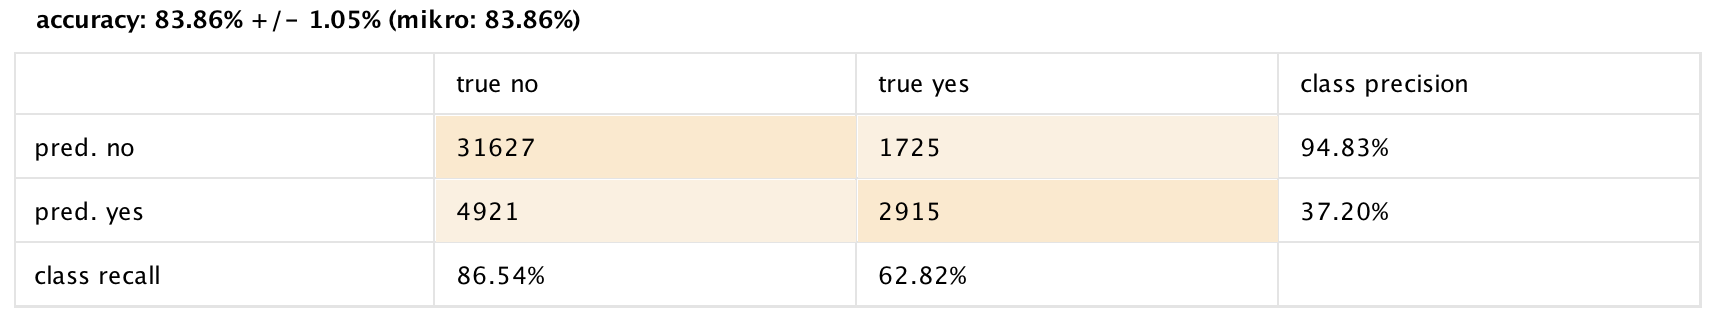
\includegraphics[width=\textwidth,height=\textheight,keepaspectratio]{rand-forest}
  %\includegraphics[width=\textwidth,height=\textheight,keepaspectratio]{}
\end{frame}

\begin{frame}
	\frametitle{Random Forest}
  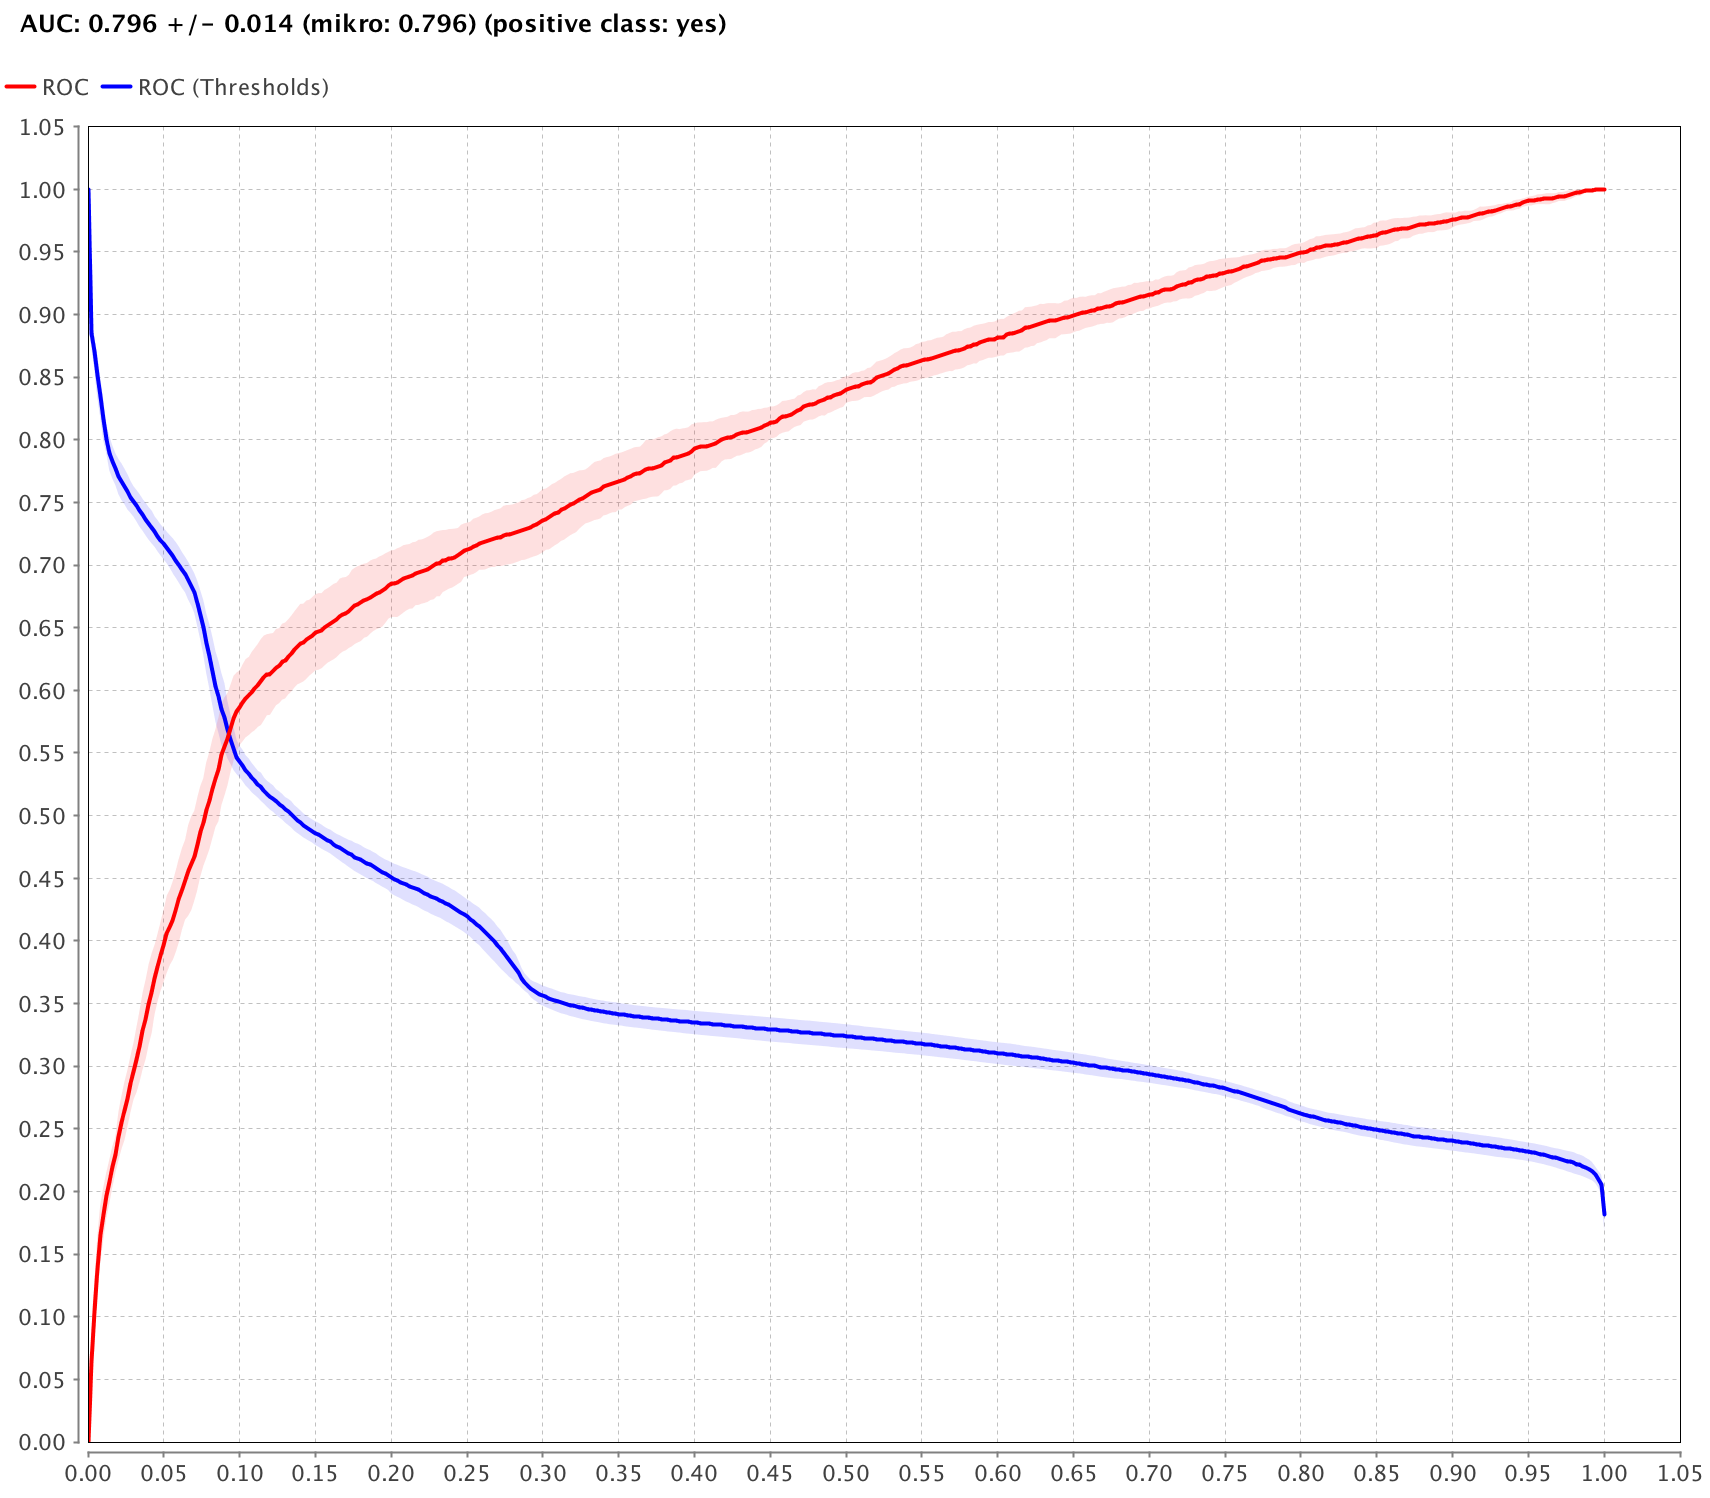
\includegraphics[width=\textwidth,height=\textheight,keepaspectratio]{rand-forest-roc}
  %\includegraphics[width=\textwidth,height=\textheight,keepaspectratio]{}
\end{frame}

%----------------------------------------------------------------------------------------

\end{document} 